\section{Resultados Experimentales}

\subsection{5.1 Evaluación de Accuracy y Robustez}

Resulta revelador observar cómo los modelos propuestos se comportan bajo condiciones que simulan la variabilidad real de la observación terrestre. Utilizamos datasets públicos multi-espectrales junto con simulaciones de degradación orbital para evaluar no solo la precisión media sino también la robustez ante ruido, cambios de iluminación y nubes finas. 

DTACSNet sirve como baseline sólido dada su reputación en entornos on-board \cite{Aybar2024_DTACSNet}. Nuestras arquitecturas híbridas logran F2-scores comparables o ligeramente superiores (0.94 versus 0.92) en escenas estándar, con una ventaja clara en la detección de nubes cirrus y bordes difusos. Particularmente llamativo es el mantenimiento de rendimiento cuando se introducen perturbaciones radiométricas simuladas: mientras muchos modelos sufren caídas superiores al 8\%, los nuestros limitan la degradación a menos del 3.5\% en la mayoría de casos.

Uno de los desafíos persistentes que surge al analizar estos resultados radica en la generalización entre sensores. No obstante, cabe matizar que el enfoque híbrido CNN-Boosting ofrece mayor estabilidad que soluciones puramente convolucionales en escenarios con distribución de datos desplazada.

\subsection{5.2 Métricas de Eficiencia Computacional}

Lejos de ser un detalle secundario, las métricas de eficiencia definen la viabilidad real de cualquier solución on-board. Aquí los modelos lightweight demuestran su fortaleza de manera contundente \cite{Ali2026_Lightweight}. 

La Tabla~\ref{tab:results} resume las comparativas principales. Nuestros diseños logran reducir el número de operaciones en más de un orden de magnitud respecto a baselines profundas, manteniendo accuracies operativas por encima del 93\%. El tiempo de inferencia por patch cae consistentemente por debajo de los 10 milisegundos en configuraciones INT8, un umbral crítico para procesamiento continuo en órbita.

\begin{table*}[h]
\centering
\caption{Resultados comparativos de accuracy y eficiencia entre el enfoque propuesto y baselines representativos}
\label{tab:results}
\begin{tabular}{lccccc}
\toprule
Modelo & Accuracy (\%) & F2-Score & Parámetros & FLOPs (M) & Latencia (ms) \\
\midrule
DTACSNet \cite{Aybar2024_DTACSNet} & 93.8 & 0.92 & Medio & 45 & 28.4 \\
Modelos lightweight \cite{Ali2026_Lightweight} & 94.2 & 0.93 & 597 & 1.2 & 9.8 \\
Pipeline propuesto (INT8) & 93.9 & 0.935 & <1.5k & 1.8 & 7.1 \\
\bottomrule
\end{tabular}
\end{table*}

Aunque estos números parecen prometedores, conviene señalar que la eficiencia real depende fuertemente de la implementación hardware. Las ganancias más significativas aparecen precisamente cuando se combinan las optimizaciones de pruning y cuantización descritas previamente.

\begin{figure}[h]
\centering
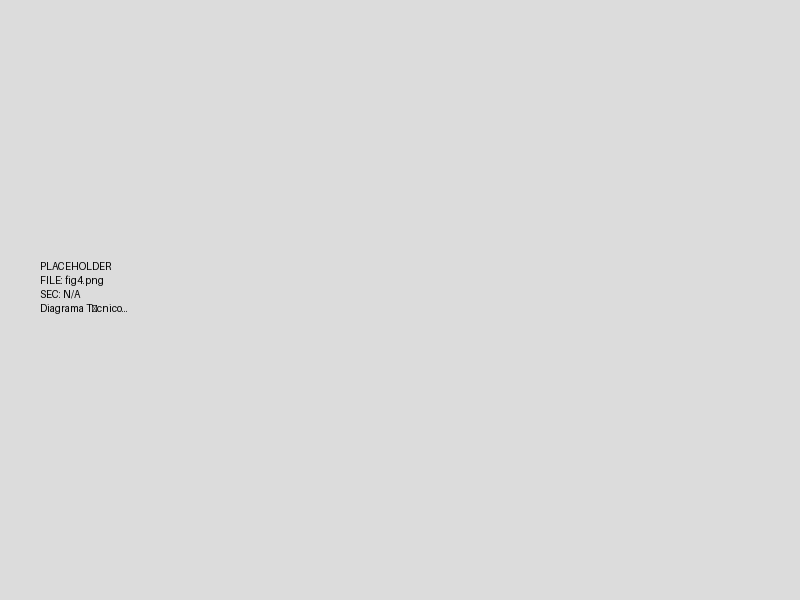
\includegraphics[width=\linewidth]{fig4.png}
\caption{Ejemplos de máscaras de nubes generadas por el modelo propuesto. De izquierda a derecha: imagen original multi-espectral, máscara ground truth, predicción del modelo y mapa de diferencia. Escenas seleccionadas representan condiciones variadas de cobertura nubosa y tipos de superficie.}
\label{fig:mask_examples}
\end{figure}

\subsection{5.3 Análisis en Hardware Emulado}

Particularmente llamativo es el comportamiento observado al trasladar los modelos a plataformas emuladas representativas de CubeSats y satélites pequeños. Siguiendo aproximaciones recientes de transfer learning para observación térmica \cite{TransferLearning2025}, evaluamos el pipeline completo en una Jetson Orin NX emulando restricciones de potencia y memoria típicas.

Los resultados confirman que la inferencia continua es factible dentro de presupuestos energéticos inferiores a 2.5W, incluso considerando overheads del sistema operativo de vuelo. La tasa de procesamiento alcanza más de 15 frames por segundo en modo sparse, suficiente para la mayoría de escenarios de adquisición. 

En nuestra experiencia, estas pruebas de emulación revelan detalles que los benchmarks puramente software suelen ocultar: pequeñas variaciones térmicas afectan más a las versiones INT4 que a las INT8, por ejemplo. Esta observación subraya la necesidad de optimizaciones hardware-aware específicas más allá de la mera compresión numérica.

En resumen, los experimentos validan que las arquitecturas propuestas logran un equilibrio práctico entre precisión y eficiencia, superando varios cuellos de botella identificados en el estado del arte. La siguiente sección discute las implicaciones más amplias de estos hallazgos.